% Options for packages loaded elsewhere
\PassOptionsToPackage{unicode}{hyperref}
\PassOptionsToPackage{hyphens}{url}
%
\documentclass[
  12pt,
]{article}
\title{Air Quality in Ukraine post Ukraine-Russia Dispute}
\usepackage{etoolbox}
\makeatletter
\providecommand{\subtitle}[1]{% add subtitle to \maketitle
  \apptocmd{\@title}{\par {\large #1 \par}}{}{}
}
\makeatother
\subtitle{Web address for GitHub repository}
\author{Curly Girlies: Shirley Fontanié, Rachel Gordon, and Julia
Weinberg}
\date{}

\usepackage{amsmath,amssymb}
\usepackage{lmodern}
\usepackage{iftex}
\ifPDFTeX
  \usepackage[T1]{fontenc}
  \usepackage[utf8]{inputenc}
  \usepackage{textcomp} % provide euro and other symbols
\else % if luatex or xetex
  \usepackage{unicode-math}
  \defaultfontfeatures{Scale=MatchLowercase}
  \defaultfontfeatures[\rmfamily]{Ligatures=TeX,Scale=1}
  \setmainfont[]{Times New Roman}
\fi
% Use upquote if available, for straight quotes in verbatim environments
\IfFileExists{upquote.sty}{\usepackage{upquote}}{}
\IfFileExists{microtype.sty}{% use microtype if available
  \usepackage[]{microtype}
  \UseMicrotypeSet[protrusion]{basicmath} % disable protrusion for tt fonts
}{}
\makeatletter
\@ifundefined{KOMAClassName}{% if non-KOMA class
  \IfFileExists{parskip.sty}{%
    \usepackage{parskip}
  }{% else
    \setlength{\parindent}{0pt}
    \setlength{\parskip}{6pt plus 2pt minus 1pt}}
}{% if KOMA class
  \KOMAoptions{parskip=half}}
\makeatother
\usepackage{xcolor}
\IfFileExists{xurl.sty}{\usepackage{xurl}}{} % add URL line breaks if available
\IfFileExists{bookmark.sty}{\usepackage{bookmark}}{\usepackage{hyperref}}
\hypersetup{
  pdftitle={Air Quality in Ukraine post Ukraine-Russia Dispute},
  pdfauthor={Curly Girlies: Shirley Fontanié, Rachel Gordon, and Julia Weinberg},
  hidelinks,
  pdfcreator={LaTeX via pandoc}}
\urlstyle{same} % disable monospaced font for URLs
\usepackage[margin=2.54cm]{geometry}
\usepackage{color}
\usepackage{fancyvrb}
\newcommand{\VerbBar}{|}
\newcommand{\VERB}{\Verb[commandchars=\\\{\}]}
\DefineVerbatimEnvironment{Highlighting}{Verbatim}{commandchars=\\\{\}}
% Add ',fontsize=\small' for more characters per line
\usepackage{framed}
\definecolor{shadecolor}{RGB}{248,248,248}
\newenvironment{Shaded}{\begin{snugshade}}{\end{snugshade}}
\newcommand{\AlertTok}[1]{\textcolor[rgb]{0.94,0.16,0.16}{#1}}
\newcommand{\AnnotationTok}[1]{\textcolor[rgb]{0.56,0.35,0.01}{\textbf{\textit{#1}}}}
\newcommand{\AttributeTok}[1]{\textcolor[rgb]{0.77,0.63,0.00}{#1}}
\newcommand{\BaseNTok}[1]{\textcolor[rgb]{0.00,0.00,0.81}{#1}}
\newcommand{\BuiltInTok}[1]{#1}
\newcommand{\CharTok}[1]{\textcolor[rgb]{0.31,0.60,0.02}{#1}}
\newcommand{\CommentTok}[1]{\textcolor[rgb]{0.56,0.35,0.01}{\textit{#1}}}
\newcommand{\CommentVarTok}[1]{\textcolor[rgb]{0.56,0.35,0.01}{\textbf{\textit{#1}}}}
\newcommand{\ConstantTok}[1]{\textcolor[rgb]{0.00,0.00,0.00}{#1}}
\newcommand{\ControlFlowTok}[1]{\textcolor[rgb]{0.13,0.29,0.53}{\textbf{#1}}}
\newcommand{\DataTypeTok}[1]{\textcolor[rgb]{0.13,0.29,0.53}{#1}}
\newcommand{\DecValTok}[1]{\textcolor[rgb]{0.00,0.00,0.81}{#1}}
\newcommand{\DocumentationTok}[1]{\textcolor[rgb]{0.56,0.35,0.01}{\textbf{\textit{#1}}}}
\newcommand{\ErrorTok}[1]{\textcolor[rgb]{0.64,0.00,0.00}{\textbf{#1}}}
\newcommand{\ExtensionTok}[1]{#1}
\newcommand{\FloatTok}[1]{\textcolor[rgb]{0.00,0.00,0.81}{#1}}
\newcommand{\FunctionTok}[1]{\textcolor[rgb]{0.00,0.00,0.00}{#1}}
\newcommand{\ImportTok}[1]{#1}
\newcommand{\InformationTok}[1]{\textcolor[rgb]{0.56,0.35,0.01}{\textbf{\textit{#1}}}}
\newcommand{\KeywordTok}[1]{\textcolor[rgb]{0.13,0.29,0.53}{\textbf{#1}}}
\newcommand{\NormalTok}[1]{#1}
\newcommand{\OperatorTok}[1]{\textcolor[rgb]{0.81,0.36,0.00}{\textbf{#1}}}
\newcommand{\OtherTok}[1]{\textcolor[rgb]{0.56,0.35,0.01}{#1}}
\newcommand{\PreprocessorTok}[1]{\textcolor[rgb]{0.56,0.35,0.01}{\textit{#1}}}
\newcommand{\RegionMarkerTok}[1]{#1}
\newcommand{\SpecialCharTok}[1]{\textcolor[rgb]{0.00,0.00,0.00}{#1}}
\newcommand{\SpecialStringTok}[1]{\textcolor[rgb]{0.31,0.60,0.02}{#1}}
\newcommand{\StringTok}[1]{\textcolor[rgb]{0.31,0.60,0.02}{#1}}
\newcommand{\VariableTok}[1]{\textcolor[rgb]{0.00,0.00,0.00}{#1}}
\newcommand{\VerbatimStringTok}[1]{\textcolor[rgb]{0.31,0.60,0.02}{#1}}
\newcommand{\WarningTok}[1]{\textcolor[rgb]{0.56,0.35,0.01}{\textbf{\textit{#1}}}}
\usepackage{longtable,booktabs,array}
\usepackage{calc} % for calculating minipage widths
% Correct order of tables after \paragraph or \subparagraph
\usepackage{etoolbox}
\makeatletter
\patchcmd\longtable{\par}{\if@noskipsec\mbox{}\fi\par}{}{}
\makeatother
% Allow footnotes in longtable head/foot
\IfFileExists{footnotehyper.sty}{\usepackage{footnotehyper}}{\usepackage{footnote}}
\makesavenoteenv{longtable}
\usepackage{graphicx}
\makeatletter
\def\maxwidth{\ifdim\Gin@nat@width>\linewidth\linewidth\else\Gin@nat@width\fi}
\def\maxheight{\ifdim\Gin@nat@height>\textheight\textheight\else\Gin@nat@height\fi}
\makeatother
% Scale images if necessary, so that they will not overflow the page
% margins by default, and it is still possible to overwrite the defaults
% using explicit options in \includegraphics[width, height, ...]{}
\setkeys{Gin}{width=\maxwidth,height=\maxheight,keepaspectratio}
% Set default figure placement to htbp
\makeatletter
\def\fps@figure{htbp}
\makeatother
\setlength{\emergencystretch}{3em} % prevent overfull lines
\providecommand{\tightlist}{%
  \setlength{\itemsep}{0pt}\setlength{\parskip}{0pt}}
\setcounter{secnumdepth}{5}
\ifLuaTeX
  \usepackage{selnolig}  % disable illegal ligatures
\fi

\begin{document}
\maketitle

\newpage
\tableofcontents 
\newpage
\listoftables 
\newpage
\listoffigures 
\newpage

\hypertarget{rationale-and-research-questions}{%
\section{Rationale and Research
Questions}\label{rationale-and-research-questions}}

\begin{quote}
Research question: How does air quality in various Ukrainian cities
differ before and after the Ukraine-Russia dispute?\\
******* Rationale: On February 24, 2022, Russia attacked Ukraine. The
first city attacked was Lviv and Dnipro. Kyiv was hit February 24th.
\end{quote}

\newpage

\hypertarget{dataset-information}{%
\section{Dataset Information}\label{dataset-information}}

\begin{quote}
Describe sources of data here (input Julia paragraph)
\end{quote}

\begin{Shaded}
\begin{Highlighting}[]
\CommentTok{\# Initial wrangling }

\NormalTok{Ukraine\_Processed }\OtherTok{\textless{}{-}}\NormalTok{ UkraineData }\SpecialCharTok{\%\textgreater{}\%} 
  \FunctionTok{drop\_na}\NormalTok{(pm10) }\SpecialCharTok{\%\textgreater{}\%} 
  \FunctionTok{drop\_na}\NormalTok{(pm25) }

\CommentTok{\# Setting Date }

\NormalTok{Ukraine\_Processed}\SpecialCharTok{$}\NormalTok{date }\OtherTok{\textless{}{-}} \FunctionTok{as.Date}\NormalTok{(Ukraine\_Processed}\SpecialCharTok{$}\NormalTok{date, }\StringTok{"\%m/\%d/\%y"}\NormalTok{)}

\CommentTok{\# Creating subsets by city  }

\NormalTok{Dnipro\_2021 }\OtherTok{\textless{}{-}}\NormalTok{ Ukraine\_Processed }\SpecialCharTok{\%\textgreater{}\%} 
  \FunctionTok{filter}\NormalTok{(City }\SpecialCharTok{\%in\%} \StringTok{"Dnipro"}\NormalTok{)}\SpecialCharTok{\%\textgreater{}\%}
  \FunctionTok{subset}\NormalTok{(date }\SpecialCharTok{\textgreater{}} \StringTok{"2021{-}2{-}28"} \SpecialCharTok{\&}\NormalTok{ date }\SpecialCharTok{\textless{}} \StringTok{"2021{-}04{-}01"}\NormalTok{) }\SpecialCharTok{\%\textgreater{}\%}
  \FunctionTok{mutate}\NormalTok{(}\AttributeTok{Month =} \FunctionTok{month}\NormalTok{(date), }
         \AttributeTok{Day =} \FunctionTok{day}\NormalTok{(date), }
          \AttributeTok{Year =} \FunctionTok{as.factor}\NormalTok{(}\FunctionTok{year}\NormalTok{(date)))}

                
\NormalTok{Dnipro\_2022 }\OtherTok{\textless{}{-}}\NormalTok{ Ukraine\_Processed }\SpecialCharTok{\%\textgreater{}\%}
  \FunctionTok{filter}\NormalTok{(City }\SpecialCharTok{\%in\%} \StringTok{"Dnipro"}\NormalTok{)}\SpecialCharTok{\%\textgreater{}\%}
  \FunctionTok{subset}\NormalTok{(date }\SpecialCharTok{\textgreater{}} \StringTok{"2022{-}2{-}28"} \SpecialCharTok{\&}\NormalTok{ date }\SpecialCharTok{\textless{}} \StringTok{"2022{-}04{-}01"}\NormalTok{) }\SpecialCharTok{\%\textgreater{}\%}
   \FunctionTok{mutate}\NormalTok{(}\AttributeTok{Month =} \FunctionTok{month}\NormalTok{(date), }
         \AttributeTok{Day =} \FunctionTok{day}\NormalTok{(date), }
          \AttributeTok{Year =} \FunctionTok{as.factor}\NormalTok{(}\FunctionTok{year}\NormalTok{(date)))}

\NormalTok{Lviv\_2021 }\OtherTok{\textless{}{-}}\NormalTok{ Ukraine\_Processed }\SpecialCharTok{\%\textgreater{}\%} 
  \FunctionTok{filter}\NormalTok{(City }\SpecialCharTok{\%in\%} \StringTok{"Lviv"}\NormalTok{) }\SpecialCharTok{\%\textgreater{}\%}
  \FunctionTok{subset}\NormalTok{(date }\SpecialCharTok{\textgreater{}} \StringTok{"2021{-}2{-}28"} \SpecialCharTok{\&}\NormalTok{ date }\SpecialCharTok{\textless{}} \StringTok{"2021{-}04{-}01"}\NormalTok{) }\SpecialCharTok{\%\textgreater{}\%}
  \FunctionTok{mutate}\NormalTok{(}\AttributeTok{Month =} \FunctionTok{month}\NormalTok{(date), }
         \AttributeTok{Day =} \FunctionTok{day}\NormalTok{(date), }
          \AttributeTok{Year =} \FunctionTok{as.factor}\NormalTok{(}\FunctionTok{year}\NormalTok{(date)))}

\NormalTok{Lviv\_2022 }\OtherTok{\textless{}{-}}\NormalTok{ Ukraine\_Processed }\SpecialCharTok{\%\textgreater{}\%} 
  \FunctionTok{filter}\NormalTok{(City }\SpecialCharTok{\%in\%} \StringTok{"Lviv"}\NormalTok{) }\SpecialCharTok{\%\textgreater{}\%}
  \FunctionTok{subset}\NormalTok{(date }\SpecialCharTok{\textgreater{}} \StringTok{"2022{-}2{-}28"} \SpecialCharTok{\&}\NormalTok{ date }\SpecialCharTok{\textless{}} \StringTok{"2022{-}04{-}01"}\NormalTok{) }\SpecialCharTok{\%\textgreater{}\%}
  \FunctionTok{mutate}\NormalTok{(}\AttributeTok{Month =} \FunctionTok{month}\NormalTok{(date), }
         \AttributeTok{Day =} \FunctionTok{day}\NormalTok{(date), }
          \AttributeTok{Year =} \FunctionTok{as.factor}\NormalTok{(}\FunctionTok{year}\NormalTok{(date)))}

\NormalTok{FULL\_DNIPRO }\OtherTok{\textless{}{-}} \FunctionTok{bind\_rows}\NormalTok{(Dnipro\_2021,Dnipro\_2022)}

\NormalTok{FULL\_LVIV }\OtherTok{\textless{}{-}} \FunctionTok{bind\_rows}\NormalTok{(Lviv\_2021,Lviv\_2022)}
\end{Highlighting}
\end{Shaded}

\begin{quote}
Explain data wrangling process here (shirley do this)
\end{quote}

\begin{longtable}[]{@{}ll@{}}
\toprule
Data File Name & Description \\
\midrule
\endhead
UkraineData & (Raw) Ukraine air quality data \\
Ukraine\_Processed & (Processed) Ukraine air quality data, w/o na's \\
Dnipro & (Processed) Dnipro air quality data, w/ PM2.5 and PM10 \\
Lviv & (Processed) Lviv air quality data w/ PM2.5 and PM10 \\
\bottomrule
\end{longtable}

\newpage

\hypertarget{exploratory-analysis}{%
\section{Exploratory Analysis}\label{exploratory-analysis}}

\begin{Shaded}
\begin{Highlighting}[]
\CommentTok{\# DNIPRO PM2.5}

\CommentTok{\#group=as.Date(year(Dnipro\_2021$date)), color =as.Date(year(Dnipro\_2021$date)))}
\CommentTok{\#aes(month(date, label = TRUE, abbr = TRUE)) }

\NormalTok{PM25\_Dnipro\_PLOT }\OtherTok{\textless{}{-}} 
  \FunctionTok{ggplot}\NormalTok{(FULL\_DNIPRO) }\SpecialCharTok{+} 
\NormalTok{  (}\FunctionTok{aes}\NormalTok{(}\AttributeTok{x =}\NormalTok{ Day, }\AttributeTok{y =}\NormalTok{ pm25, }\AttributeTok{color =}\NormalTok{ Year))}\SpecialCharTok{+} 
  \FunctionTok{geom\_line}\NormalTok{()}\SpecialCharTok{+}  
  \FunctionTok{geom\_point}\NormalTok{()}\SpecialCharTok{+}
  \FunctionTok{labs}\NormalTok{(}\AttributeTok{x=} \StringTok{"Date"}\NormalTok{, }\AttributeTok{y =} \StringTok{"PM2.5"}\NormalTok{,}
       \AttributeTok{title =} \StringTok{" Observing PM2.5 Values in Dnipro, Ukraine"}\NormalTok{)}
\FunctionTok{print}\NormalTok{(PM25\_Dnipro\_PLOT)}
\end{Highlighting}
\end{Shaded}

\begin{figure}
\centering
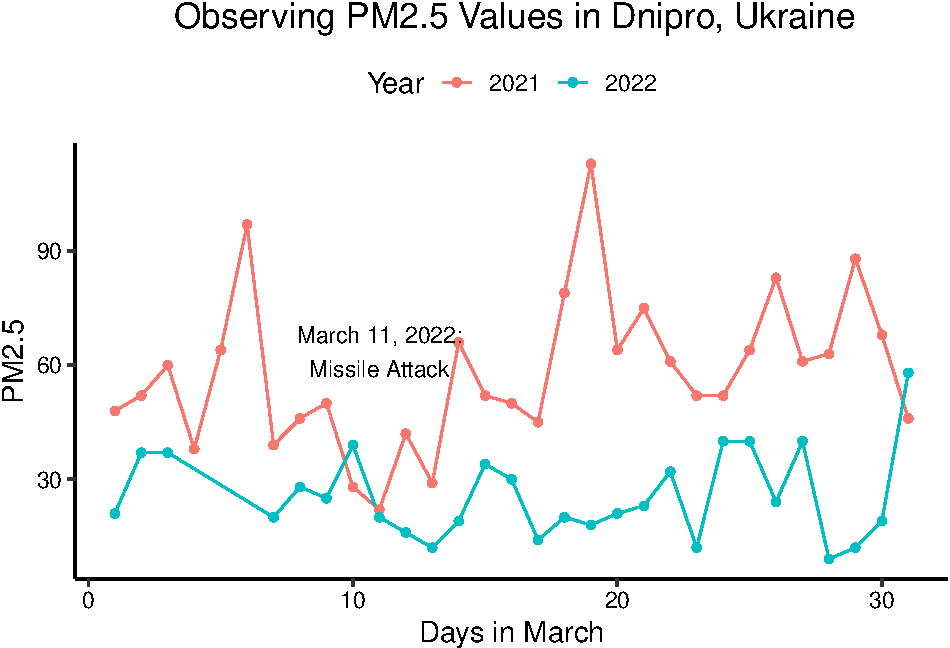
\includegraphics{Fontanie_Gordon_Weinberg_Project_files/figure-latex/Plotting.PM25-1.pdf}
\caption{Comparing PM2.5 in Dnipro and Lviv, Ukraine}
\end{figure}

\begin{Shaded}
\begin{Highlighting}[]
  \CommentTok{\#annotate(geom = "text", x = as.Date("2022{-}03{-}11"), y = 50, label ="March 11, 2022:")+ }
  \CommentTok{\#annotate(geom = "text", x = as.Date("2022{-}03{-}11"), y = 45, label ="Missile Attack")}




\CommentTok{\# LVIV PM2.5}
\NormalTok{PM25\_Lviv\_PLOT }\OtherTok{\textless{}{-}} 
  \FunctionTok{ggplot}\NormalTok{(FULL\_LVIV) }\SpecialCharTok{+} 
\NormalTok{(}\FunctionTok{aes}\NormalTok{(}\AttributeTok{x =}\NormalTok{ Day, }\AttributeTok{y =}\NormalTok{ pm25, }\AttributeTok{color =}\NormalTok{ Year)) }\SpecialCharTok{+} 
              \FunctionTok{geom\_line}\NormalTok{()}\SpecialCharTok{+}  
  \FunctionTok{geom\_point}\NormalTok{()}\SpecialCharTok{+}
  \FunctionTok{labs}\NormalTok{(}\AttributeTok{x =} \StringTok{"Date"}\NormalTok{, }\AttributeTok{y=} \StringTok{"PM2.5"}\NormalTok{,}
       \AttributeTok{title =} \StringTok{"Observing PM2.5 Values in Lviv Ukraine"}\NormalTok{)}
\FunctionTok{print}\NormalTok{(PM25\_Lviv\_PLOT)}
\end{Highlighting}
\end{Shaded}

\begin{figure}
\centering
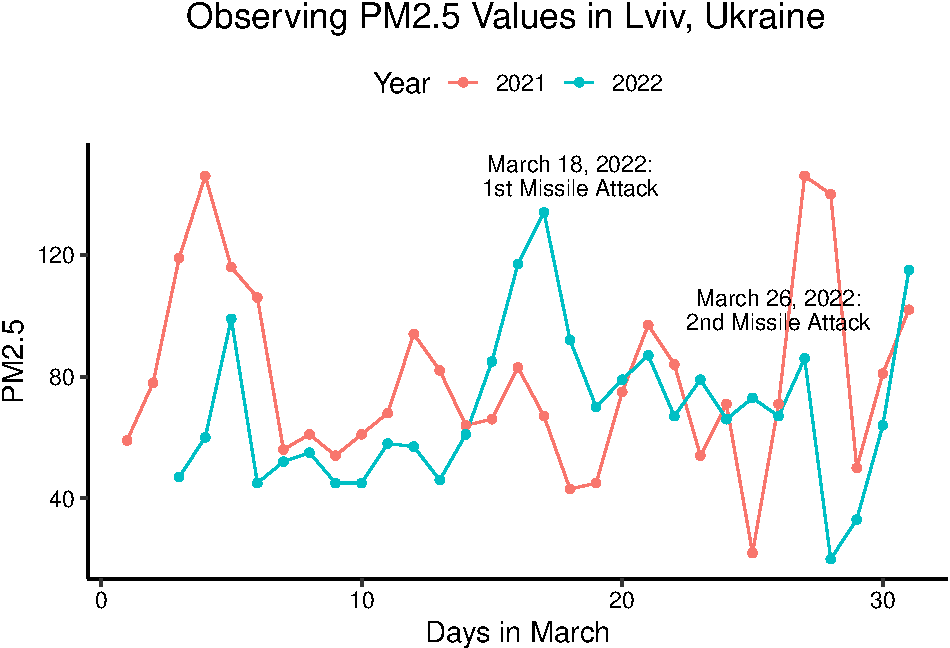
\includegraphics{Fontanie_Gordon_Weinberg_Project_files/figure-latex/Plotting.PM25-2.pdf}
\caption{Comparing PM2.5 in Dnipro and Lviv, Ukraine}
\end{figure}

\begin{Shaded}
\begin{Highlighting}[]
  \CommentTok{\#scale\_x\_date(limits = as.Date(c("2022{-}03{-}01", "2022{-}03{-}31")))+ }
  \CommentTok{\#xlab("Date")+ }
  \CommentTok{\#ylab("PM2.5")+ }
 \CommentTok{\# labs(title = "        Observing PM2.5 Values in Lviv, Ukraine")+}
  \CommentTok{\#ylim(0,180)+}
 \CommentTok{\# annotate(geom = "text", x = as.Date("2022{-}03{-}18"), y = 165, label ="March 18, 2022:")+ }
  \CommentTok{\#annotate(geom = "text", x = as.Date("2022{-}03{-}18"), y = 155, label ="1st Missile Attack")+ }
  \CommentTok{\#annotate(geom = "text", x = as.Date("2022{-}03{-}26"), y = 110, label ="March 26, 2022:")+ }
  \CommentTok{\#annotate(geom = "text", x = as.Date("2022{-}03{-}26"), y = 100, label ="2nd Missile Attack")}
\end{Highlighting}
\end{Shaded}

\begin{Shaded}
\begin{Highlighting}[]
\CommentTok{\#DNIPRO PM2.5}
\NormalTok{PM10\_Dnipro\_PLOT }\OtherTok{\textless{}{-}}\FunctionTok{ggplot}\NormalTok{(FULL\_DNIPRO) }\SpecialCharTok{+} 
\NormalTok{  (}\FunctionTok{aes}\NormalTok{(}\AttributeTok{x =}\NormalTok{ Day, }\AttributeTok{y =}\NormalTok{ pm10, }\AttributeTok{color =}\NormalTok{ Year))}\SpecialCharTok{+} 
  \FunctionTok{geom\_line}\NormalTok{()}\SpecialCharTok{+}  
  \FunctionTok{geom\_point}\NormalTok{()}\SpecialCharTok{+}
  \FunctionTok{labs}\NormalTok{(}\AttributeTok{x=} \StringTok{"Date"}\NormalTok{, }\AttributeTok{y =} \StringTok{"PM10"}\NormalTok{,}
       \AttributeTok{title =} \StringTok{" Observing PM10 Values in Dnipro, Ukraine"}\NormalTok{)}
\FunctionTok{print}\NormalTok{(PM10\_Dnipro\_PLOT) }
\end{Highlighting}
\end{Shaded}

\begin{figure}
\centering
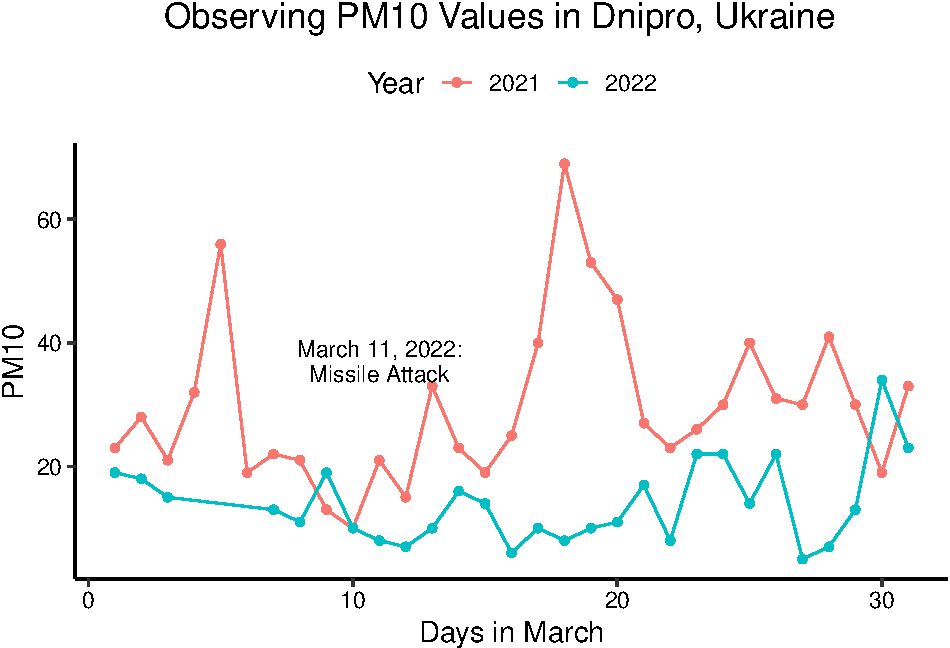
\includegraphics{Fontanie_Gordon_Weinberg_Project_files/figure-latex/Plotting PM10-1.pdf}
\caption{Comparing PM10 in Dnipro and Lviv, Ukraine}
\end{figure}

\begin{Shaded}
\begin{Highlighting}[]
            \CommentTok{\#  geom\_line()+  }
 \CommentTok{\# geom\_point()+}
  \CommentTok{\#scale\_x\_date(limits = as.Date(c("2022{-}03{-}01", "2022{-}03{-}31")))+ }
  \CommentTok{\#xlab("Date")+ }
  \CommentTok{\#ylab("PM10")+ }
  \CommentTok{\#labs(title = "        Observing PM10 Values in Dnipro, Ukraine")+}
  \CommentTok{\#ylim(0,40)+}
  \CommentTok{\#annotate(geom = "text", x = as.Date("2022{-}03{-}11"), y = 25, label ="March 11, 2022:")+ }
  \CommentTok{\#annotate(geom = "text", x = as.Date("2022{-}03{-}11"), y = 23, label ="Missile Attack")}
  


\CommentTok{\#LVIV PM10}
\NormalTok{PM10\_Lviv\_PLOT }\OtherTok{\textless{}{-}}
  \FunctionTok{ggplot}\NormalTok{(FULL\_LVIV) }\SpecialCharTok{+} 
\NormalTok{(}\FunctionTok{aes}\NormalTok{(}\AttributeTok{x =}\NormalTok{ Day, }\AttributeTok{y =}\NormalTok{ pm10, }\AttributeTok{color =}\NormalTok{ Year)) }\SpecialCharTok{+} 
              \FunctionTok{geom\_line}\NormalTok{()}\SpecialCharTok{+}  
  \FunctionTok{geom\_point}\NormalTok{()}\SpecialCharTok{+}
  \FunctionTok{labs}\NormalTok{(}\AttributeTok{x =} \StringTok{"Date"}\NormalTok{, }\AttributeTok{y=} \StringTok{"PM10"}\NormalTok{,}
       \AttributeTok{title =} \StringTok{"Observing PM10 Values in Lviv Ukraine"}\NormalTok{)  }
\FunctionTok{print}\NormalTok{(PM10\_Lviv\_PLOT)}
\end{Highlighting}
\end{Shaded}

\begin{figure}
\centering
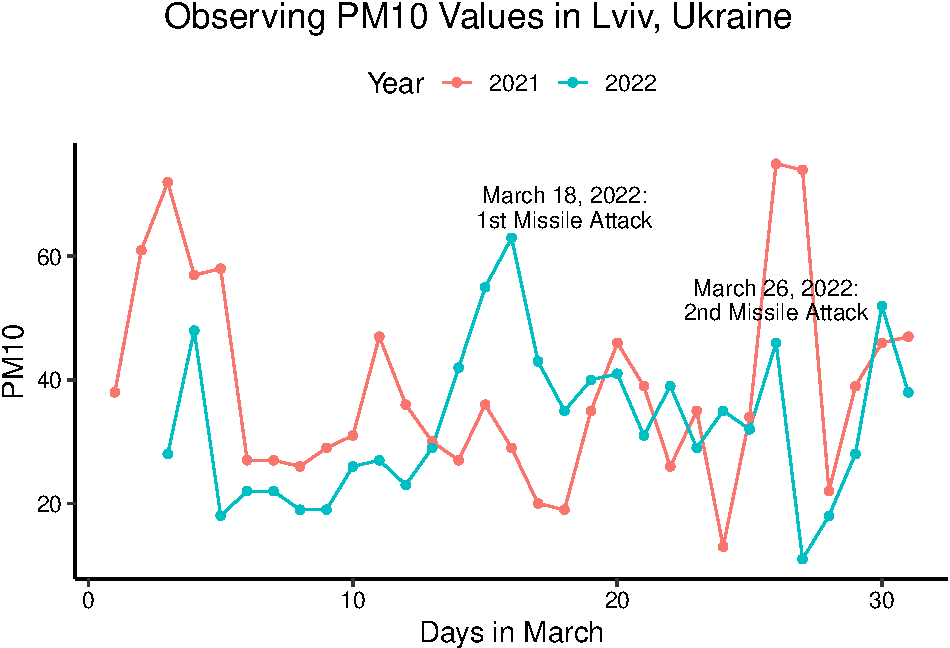
\includegraphics{Fontanie_Gordon_Weinberg_Project_files/figure-latex/Plotting PM10-2.pdf}
\caption{Comparing PM10 in Dnipro and Lviv, Ukraine}
\end{figure}

\begin{Shaded}
\begin{Highlighting}[]
  \CommentTok{\#geom\_point()+}
  \CommentTok{\#scale\_x\_date(limits = as.Date(c("2022{-}03{-}01", "2022{-}03{-}31")))+ }
  \CommentTok{\#xlab("Date")+ }
  \CommentTok{\#ylab("PM10")+ }
  \CommentTok{\#labs(title = "        Observing PM10 Values in Lviv, Ukraine")+}
  \CommentTok{\#ylim(0,75)+}
  \CommentTok{\#annotate(geom = "text", x = as.Date("2022{-}03{-}18"), y = 70, label ="March 18, 2022:")+ }
  \CommentTok{\#annotate(geom = "text", x = as.Date("2022{-}03{-}18"), y = 66, label ="1st Missile Attack")+ }
  \CommentTok{\#annotate(geom = "text", x = as.Date("2022{-}03{-}26"), y = 60, label ="March 26, 2022:")+ }
  \CommentTok{\#annotate(geom = "text", x = as.Date("2022{-}03{-}26"), y = 56, label ="2nd Missile Attack")}
\end{Highlighting}
\end{Shaded}

\begin{Shaded}
\begin{Highlighting}[]
\NormalTok{FULL\_Air\_quality }\OtherTok{\textless{}{-}} \FunctionTok{bind\_rows}\NormalTok{(Dnipro\_2022,Lviv\_2022)}

\NormalTok{PM25\_Lviv\_and\_Dnipro\_PLOT }\OtherTok{\textless{}{-}}
  \FunctionTok{ggplot}\NormalTok{(FULL\_Air\_quality) }\SpecialCharTok{+} 
\NormalTok{(}\FunctionTok{aes}\NormalTok{(}\AttributeTok{x =}\NormalTok{ Day, }\AttributeTok{y =}\NormalTok{ pm25, }\AttributeTok{color =}\NormalTok{ City)) }\SpecialCharTok{+} 
              \FunctionTok{geom\_line}\NormalTok{()}\SpecialCharTok{+}  
  \FunctionTok{geom\_point}\NormalTok{()}\SpecialCharTok{+}
  \FunctionTok{labs}\NormalTok{(}\AttributeTok{x =} \StringTok{"Date"}\NormalTok{, }\AttributeTok{y=} \StringTok{"PM25"}\NormalTok{,}
       \AttributeTok{title =} \StringTok{"Observing PM25 Values in 2022 Lviv and Dnipro Ukraine"}\NormalTok{)  }
\FunctionTok{print}\NormalTok{(PM25\_Lviv\_and\_Dnipro\_PLOT)}
\end{Highlighting}
\end{Shaded}

\begin{figure}
\centering
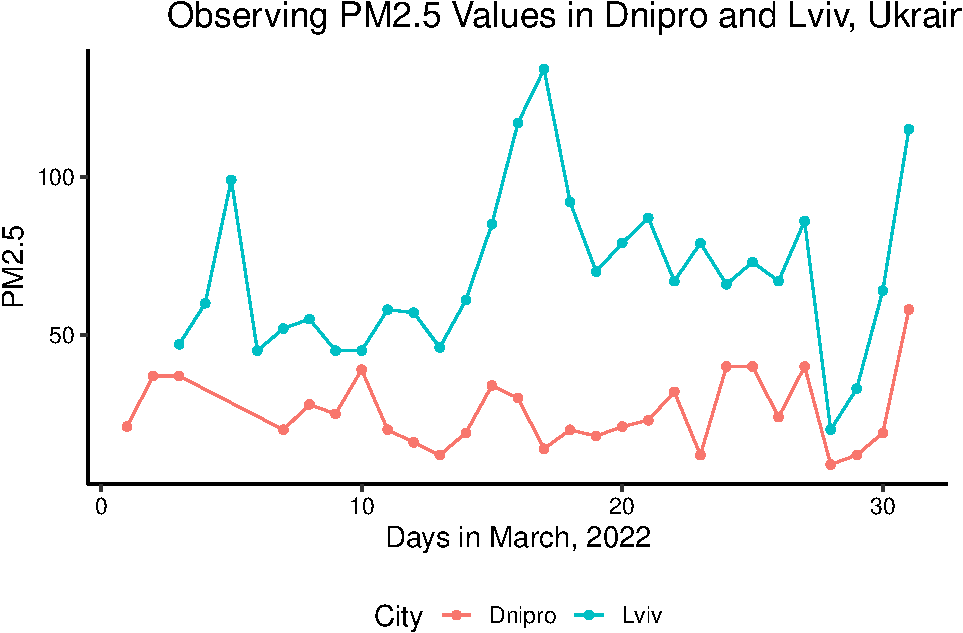
\includegraphics{Fontanie_Gordon_Weinberg_Project_files/figure-latex/Plotting Lviv vs Dnipro-1.pdf}
\caption{Comparing Air Pollution in Lviv vs Dnipro}
\end{figure}

\begin{Shaded}
\begin{Highlighting}[]
\NormalTok{PM10\_Lviv\_and\_Dnipro\_PLOT }\OtherTok{\textless{}{-}}
  \FunctionTok{ggplot}\NormalTok{(FULL\_Air\_quality) }\SpecialCharTok{+} 
\NormalTok{(}\FunctionTok{aes}\NormalTok{(}\AttributeTok{x =}\NormalTok{ Day, }\AttributeTok{y =}\NormalTok{ pm10, }\AttributeTok{color =}\NormalTok{ City)) }\SpecialCharTok{+} 
              \FunctionTok{geom\_line}\NormalTok{()}\SpecialCharTok{+}  
  \FunctionTok{geom\_point}\NormalTok{()}\SpecialCharTok{+}
  \FunctionTok{labs}\NormalTok{(}\AttributeTok{x =} \StringTok{"Date"}\NormalTok{, }\AttributeTok{y=} \StringTok{"PM10"}\NormalTok{,}
       \AttributeTok{title =} \StringTok{"Observing PM10 Values in 2022 Lviv and Dnipro Ukraine"}\NormalTok{)  }
\FunctionTok{print}\NormalTok{(PM10\_Lviv\_and\_Dnipro\_PLOT)}
\end{Highlighting}
\end{Shaded}

\begin{figure}
\centering
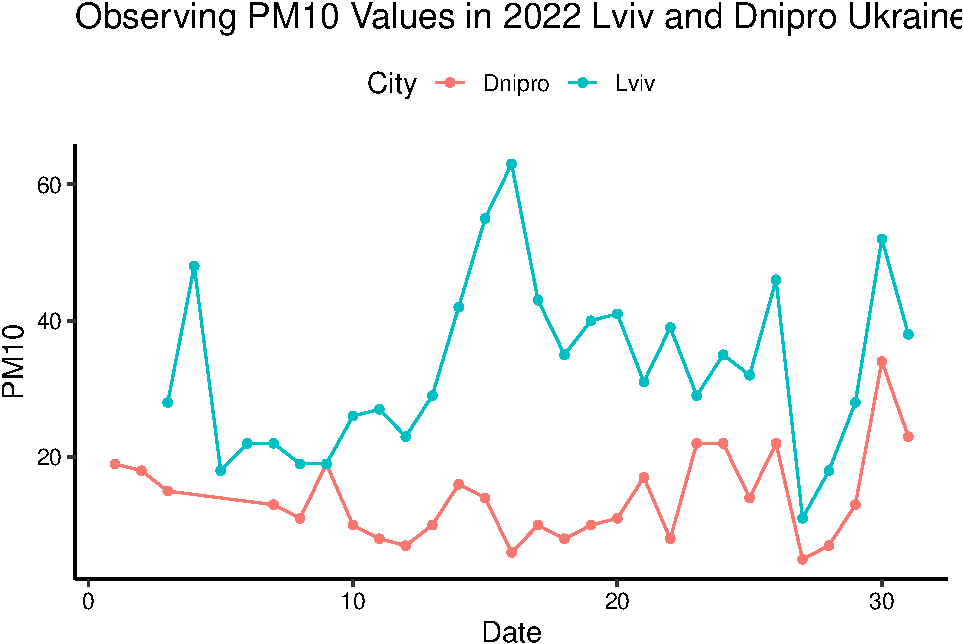
\includegraphics{Fontanie_Gordon_Weinberg_Project_files/figure-latex/Plotting Lviv vs Dnipro-2.pdf}
\caption{Comparing Air Pollution in Lviv vs Dnipro}
\end{figure}

\newpage

\hypertarget{analysis}{%
\section{Analysis}\label{analysis}}

\begin{Shaded}
\begin{Highlighting}[]
\CommentTok{\#after doing all these anovas i realized im not sure what this is really telling us and i think they might be super uncessary so i did an lm analysis in the code chunk below}

\NormalTok{lviv.pm25.anova }\OtherTok{\textless{}{-}} \FunctionTok{aov}\NormalTok{(}\AttributeTok{data =}\NormalTok{ FULL\_LVIV , pm25 }\SpecialCharTok{\textasciitilde{}}\NormalTok{ Year)}
\FunctionTok{summary}\NormalTok{(lviv.pm25.anova)}
\end{Highlighting}
\end{Shaded}

\begin{verbatim}
##             Df Sum Sq Mean Sq F value Pr(>F)
## Year         1   1585  1584.5   1.988  0.164
## Residuals   58  46232   797.1
\end{verbatim}

\begin{Shaded}
\begin{Highlighting}[]
\NormalTok{lviv.pm10.anova }\OtherTok{\textless{}{-}} \FunctionTok{aov}\NormalTok{(}\AttributeTok{data =}\NormalTok{ FULL\_LVIV , pm10 }\SpecialCharTok{\textasciitilde{}}\NormalTok{ Year)}
\FunctionTok{summary}\NormalTok{(lviv.pm10.anova)}
\end{Highlighting}
\end{Shaded}

\begin{verbatim}
##             Df Sum Sq Mean Sq F value Pr(>F)
## Year         1    482   482.2   2.281  0.136
## Residuals   58  12262   211.4
\end{verbatim}

\begin{Shaded}
\begin{Highlighting}[]
\NormalTok{dnipro.pm25.anova }\OtherTok{\textless{}{-}} \FunctionTok{aov}\NormalTok{(}\AttributeTok{data =}\NormalTok{ FULL\_DNIPRO , pm25 }\SpecialCharTok{\textasciitilde{}}\NormalTok{ Year)}
\FunctionTok{summary}\NormalTok{(dnipro.pm25.anova)}
\end{Highlighting}
\end{Shaded}

\begin{verbatim}
##             Df Sum Sq Mean Sq F value   Pr(>F)    
## Year         1  15305   15305   55.92 5.07e-10 ***
## Residuals   57  15599     274                     
## ---
## Signif. codes:  0 '***' 0.001 '**' 0.01 '*' 0.05 '.' 0.1 ' ' 1
\end{verbatim}

\begin{Shaded}
\begin{Highlighting}[]
\NormalTok{dnipro.pm10.anova }\OtherTok{\textless{}{-}} \FunctionTok{aov}\NormalTok{(}\AttributeTok{data =}\NormalTok{ FULL\_DNIPRO , pm10 }\SpecialCharTok{\textasciitilde{}}\NormalTok{ Year)}
\FunctionTok{summary}\NormalTok{(dnipro.pm10.anova)}
\end{Highlighting}
\end{Shaded}

\begin{verbatim}
##             Df Sum Sq Mean Sq F value   Pr(>F)    
## Year         1   3616    3616   32.57 4.33e-07 ***
## Residuals   57   6329     111                     
## ---
## Signif. codes:  0 '***' 0.001 '**' 0.01 '*' 0.05 '.' 0.1 ' ' 1
\end{verbatim}

\begin{Shaded}
\begin{Highlighting}[]
\NormalTok{dnipro.lviv.pm25.anova }\OtherTok{\textless{}{-}} \FunctionTok{aov}\NormalTok{(}\AttributeTok{data =}\NormalTok{ FULL\_Air\_quality , pm25 }\SpecialCharTok{\textasciitilde{}}\NormalTok{ City)}
\FunctionTok{summary}\NormalTok{(dnipro.lviv.pm25.anova)}
\end{Highlighting}
\end{Shaded}

\begin{verbatim}
##             Df Sum Sq Mean Sq F value   Pr(>F)    
## City         1  26819   26819   66.65 4.72e-11 ***
## Residuals   55  22130     402                     
## ---
## Signif. codes:  0 '***' 0.001 '**' 0.01 '*' 0.05 '.' 0.1 ' ' 1
\end{verbatim}

\begin{Shaded}
\begin{Highlighting}[]
\NormalTok{dnipro.lviv.pm10.anova }\OtherTok{\textless{}{-}} \FunctionTok{aov}\NormalTok{(}\AttributeTok{data =}\NormalTok{ FULL\_Air\_quality , pm10 }\SpecialCharTok{\textasciitilde{}}\NormalTok{ City)}
\FunctionTok{summary}\NormalTok{(dnipro.lviv.pm10.anova)}
\end{Highlighting}
\end{Shaded}

\begin{verbatim}
##             Df Sum Sq Mean Sq F value   Pr(>F)    
## City         1   5180    5180   51.52 1.93e-09 ***
## Residuals   55   5530     101                     
## ---
## Signif. codes:  0 '***' 0.001 '**' 0.01 '*' 0.05 '.' 0.1 ' ' 1
\end{verbatim}

\begin{Shaded}
\begin{Highlighting}[]
\NormalTok{lviv.}\FloatTok{25.}\NormalTok{lm }\OtherTok{\textless{}{-}} \FunctionTok{lm}\NormalTok{(}\AttributeTok{data =}\NormalTok{ FULL\_LVIV, pm25 }\SpecialCharTok{\textasciitilde{}}\NormalTok{ Year) }
\FunctionTok{summary}\NormalTok{(lviv.}\FloatTok{25.}\NormalTok{lm) }
\end{Highlighting}
\end{Shaded}

\begin{verbatim}
## 
## Call:
## lm(formula = pm25 ~ Year, data = FULL_LVIV)
## 
## Residuals:
##     Min      1Q  Median      3Q     Max 
## -57.387 -18.887  -4.745  16.147  66.613 
## 
## Coefficients:
##             Estimate Std. Error t value Pr(>|t|)    
## (Intercept)   79.387      5.071   15.66   <2e-16 ***
## Year2022     -10.284      7.294   -1.41    0.164    
## ---
## Signif. codes:  0 '***' 0.001 '**' 0.01 '*' 0.05 '.' 0.1 ' ' 1
## 
## Residual standard error: 28.23 on 58 degrees of freedom
## Multiple R-squared:  0.03314,    Adjusted R-squared:  0.01647 
## F-statistic: 1.988 on 1 and 58 DF,  p-value: 0.1639
\end{verbatim}

\begin{Shaded}
\begin{Highlighting}[]
\NormalTok{lviv.}\FloatTok{10.}\NormalTok{lm }\OtherTok{\textless{}{-}} \FunctionTok{lm}\NormalTok{(}\AttributeTok{data =}\NormalTok{ FULL\_LVIV, pm10 }\SpecialCharTok{\textasciitilde{}}\NormalTok{ Year) }
\FunctionTok{summary}\NormalTok{(lviv.}\FloatTok{10.}\NormalTok{lm) }
\end{Highlighting}
\end{Shaded}

\begin{verbatim}
## 
## Call:
## lm(formula = pm10 ~ Year, data = FULL_LVIV)
## 
## Residuals:
##     Min      1Q  Median      3Q     Max 
## -25.742 -11.069  -3.242   8.013  36.258 
## 
## Coefficients:
##             Estimate Std. Error t value Pr(>|t|)    
## (Intercept)   38.742      2.611   14.84   <2e-16 ***
## Year2022      -5.673      3.756   -1.51    0.136    
## ---
## Signif. codes:  0 '***' 0.001 '**' 0.01 '*' 0.05 '.' 0.1 ' ' 1
## 
## Residual standard error: 14.54 on 58 degrees of freedom
## Multiple R-squared:  0.03784,    Adjusted R-squared:  0.02125 
## F-statistic: 2.281 on 1 and 58 DF,  p-value: 0.1364
\end{verbatim}

\begin{Shaded}
\begin{Highlighting}[]
\NormalTok{dnipro.}\FloatTok{25.}\NormalTok{lm }\OtherTok{\textless{}{-}} \FunctionTok{lm}\NormalTok{(}\AttributeTok{data =}\NormalTok{ FULL\_DNIPRO, pm25 }\SpecialCharTok{\textasciitilde{}}\NormalTok{ Year) }
\FunctionTok{summary}\NormalTok{(dnipro.}\FloatTok{25.}\NormalTok{lm) }
\end{Highlighting}
\end{Shaded}

\begin{verbatim}
## 
## Call:
## lm(formula = pm25 ~ Year, data = FULL_DNIPRO)
## 
## Residuals:
##     Min      1Q  Median      3Q     Max 
## -35.968  -9.841  -4.714   8.159  55.032 
## 
## Coefficients:
##             Estimate Std. Error t value Pr(>|t|)    
## (Intercept)   57.968      2.971  19.510  < 2e-16 ***
## Year2022     -32.253      4.313  -7.478 5.07e-10 ***
## ---
## Signif. codes:  0 '***' 0.001 '**' 0.01 '*' 0.05 '.' 0.1 ' ' 1
## 
## Residual standard error: 16.54 on 57 degrees of freedom
## Multiple R-squared:  0.4952, Adjusted R-squared:  0.4864 
## F-statistic: 55.93 on 1 and 57 DF,  p-value: 5.074e-10
\end{verbatim}

\begin{Shaded}
\begin{Highlighting}[]
\NormalTok{dnipro.}\FloatTok{10.}\NormalTok{lm }\OtherTok{\textless{}{-}} \FunctionTok{lm}\NormalTok{(}\AttributeTok{data =}\NormalTok{ FULL\_DNIPRO, pm10 }\SpecialCharTok{\textasciitilde{}}\NormalTok{ Year) }
\FunctionTok{summary}\NormalTok{(dnipro.}\FloatTok{10.}\NormalTok{lm) }
\end{Highlighting}
\end{Shaded}

\begin{verbatim}
## 
## Call:
## lm(formula = pm10 ~ Year, data = FULL_DNIPRO)
## 
## Residuals:
##     Min      1Q  Median      3Q     Max 
## -19.677  -6.677  -1.677   3.661  39.323 
## 
## Coefficients:
##             Estimate Std. Error t value Pr(>|t|)    
## (Intercept)   29.677      1.893  15.681  < 2e-16 ***
## Year2022     -15.677      2.747  -5.707 4.33e-07 ***
## ---
## Signif. codes:  0 '***' 0.001 '**' 0.01 '*' 0.05 '.' 0.1 ' ' 1
## 
## Residual standard error: 10.54 on 57 degrees of freedom
## Multiple R-squared:  0.3636, Adjusted R-squared:  0.3524 
## F-statistic: 32.57 on 1 and 57 DF,  p-value: 4.325e-07
\end{verbatim}

\begin{Shaded}
\begin{Highlighting}[]
\NormalTok{dnipro.lviv.pm25.lm }\OtherTok{\textless{}{-}} \FunctionTok{lm}\NormalTok{(}\AttributeTok{data =}\NormalTok{ FULL\_Air\_quality, pm25 }\SpecialCharTok{\textasciitilde{}}\NormalTok{ City) }
\FunctionTok{summary}\NormalTok{(dnipro.lviv.pm25.lm)}
\end{Highlighting}
\end{Shaded}

\begin{verbatim}
## 
## Call:
## lm(formula = pm25 ~ City, data = FULL_Air_quality)
## 
## Residuals:
##     Min      1Q  Median      3Q     Max 
## -49.103 -11.714  -3.103  11.286  64.897 
## 
## Coefficients:
##             Estimate Std. Error t value Pr(>|t|)    
## (Intercept)   25.714      3.791   6.783 8.54e-09 ***
## CityLviv      43.389      5.315   8.164 4.72e-11 ***
## ---
## Signif. codes:  0 '***' 0.001 '**' 0.01 '*' 0.05 '.' 0.1 ' ' 1
## 
## Residual standard error: 20.06 on 55 degrees of freedom
## Multiple R-squared:  0.5479, Adjusted R-squared:  0.5397 
## F-statistic: 66.65 on 1 and 55 DF,  p-value: 4.715e-11
\end{verbatim}

\begin{Shaded}
\begin{Highlighting}[]
\NormalTok{dnipro.lviv.pm10.lm }\OtherTok{\textless{}{-}} \FunctionTok{lm}\NormalTok{(}\AttributeTok{data =}\NormalTok{ FULL\_Air\_quality, pm10 }\SpecialCharTok{\textasciitilde{}}\NormalTok{ City) }
\FunctionTok{summary}\NormalTok{(dnipro.lviv.pm10.lm)}
\end{Highlighting}
\end{Shaded}

\begin{verbatim}
## 
## Call:
## lm(formula = pm10 ~ City, data = FULL_Air_quality)
## 
## Residuals:
##     Min      1Q  Median      3Q     Max 
## -22.069  -6.000  -1.069   5.931  29.931 
## 
## Coefficients:
##             Estimate Std. Error t value Pr(>|t|)    
## (Intercept)   14.000      1.895   7.388 8.72e-10 ***
## CityLviv      19.069      2.657   7.178 1.93e-09 ***
## ---
## Signif. codes:  0 '***' 0.001 '**' 0.01 '*' 0.05 '.' 0.1 ' ' 1
## 
## Residual standard error: 10.03 on 55 degrees of freedom
## Multiple R-squared:  0.4837, Adjusted R-squared:  0.4743 
## F-statistic: 51.52 on 1 and 55 DF,  p-value: 1.929e-09
\end{verbatim}

\begin{Shaded}
\begin{Highlighting}[]
\CommentTok{\#I\textquotesingle{}m confused if we need to upload a shapefile of ukraine so that we can make a map but maybe im really overthinking this {-} just wanted to put it as a comment here so i dont forget }

\CommentTok{\#https://simplemaps.com/data/ua{-}cities}
\CommentTok{\#we can download a csv of all the cities with lat and long from this link and we could make a map but idk if thats what you guys were thinking}
\end{Highlighting}
\end{Shaded}

\hypertarget{question-1-are-there-significant-differences-in-air-quality-levels-between-affected-ukrainian-cities-during-the-russian-invasion}{%
\subsection{Question 1: Are there significant differences in air quality
levels between affected Ukrainian cities during the Russian
invasion?}\label{question-1-are-there-significant-differences-in-air-quality-levels-between-affected-ukrainian-cities-during-the-russian-invasion}}

\hypertarget{question-2-do-air-quality-levels-worsen-in-affected-cities-around-missile-attack-events}{%
\subsection{Question 2: Do air quality levels worsen in affected cities
around missile attack
events?}\label{question-2-do-air-quality-levels-worsen-in-affected-cities-around-missile-attack-events}}

\hypertarget{question-3-are-there-significant-differences-in-air-quality-levels-in-affected-ukrainian-cities-before-and-during-the-russian-attacks}{%
\subsection{Question 3: Are there significant differences in air quality
levels in affected Ukrainian cities before and during the Russian
attacks?}\label{question-3-are-there-significant-differences-in-air-quality-levels-in-affected-ukrainian-cities-before-and-during-the-russian-attacks}}

\newpage

\hypertarget{summary-and-conclusions}{%
\section{Summary and Conclusions}\label{summary-and-conclusions}}

\newpage

\hypertarget{references}{%
\section{References}\label{references}}

\textless add references here if relevant, otherwise delete this
section\textgreater{}

\end{document}
